\documentclass[12pt]{article}

\usepackage{amsmath}
\usepackage{amssymb}
\usepackage{fancyhdr}
\usepackage{geometry}
\usepackage{graphicx}
\usepackage{mathrsfs}
\usepackage{mdframed}
\usepackage{parskip}
\usepackage{pgf}
\usepackage{siunitx}
\usepackage{tikz}

\usetikzlibrary{arrows}
\usetikzlibrary{positioning}

\geometry{margin=0.75in}
\pagestyle{fancy}
\fancyhf{}
\lhead{Integrated Math III}
\rhead{Tuesday, April 11, 2017}

\sisetup{group-separator={,}}
\DeclareSIUnit{\inch}{in}
\DeclareSIUnit{\mile}{mi}

\newcommand{\degre}{\ensuremath{^\circ}}

\begin{document}

\begin{center}
  \textbf{\Large Trigonometry of Surveying Worksheet}
\end{center}

\begin{enumerate}
  \vspace{0.4in}
\item \emph{Warm-up:} Find the area of the following triangle:
  \vspace{0.4in}
  \begin{center}
    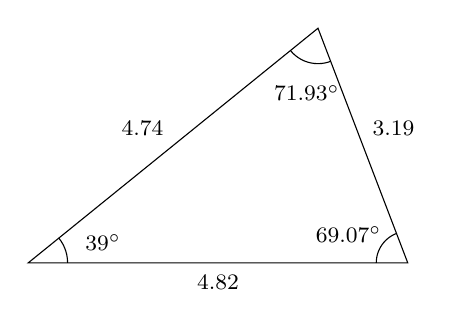
\begin{tikzpicture}
      \draw (0, 0) -- (4.82, 0) node [midway, below=0.03cm]
      {\footnotesize \SI{4.82}{\inch}} -- (3.68, 2.98) node [midway,
      above right] {\footnotesize \SI{3.19}{\inch}} -- cycle node
      [midway, above left] {\footnotesize \SI{4.74}{\inch}};

      \clip (0, 0) -- (4.82, 0) -- (3.68, 2.98) -- cycle;

      \draw (0, 0) circle (0.5cm) node [above right=0.03cm and 0.6cm]
      {\footnotesize \SI{39}{\degree}};

      \draw (4.82, 0) circle (0.4cm) node [above left=0.14cm and
      0.21cm] {\footnotesize \SI{69.07}{\degree}};

      \draw (3.68, 2.98) circle (0.45cm) node [below left=0.6cm and
      -0.4cm] {\footnotesize \SI{71.93}{\degree}};
    \end{tikzpicture}
  \end{center}
  \vspace{0.5in}
\item \emph{Surveying a canyon:} Suppose you are surveying the area
  around the Grand Canyon. Unfortunately, because of the uneven
  terrain, you can't measure accurate lengths within the region---only
  around the borders. Your team measures each segment of the border,
  and also sights the angles between each corner.

  \begin{center}
    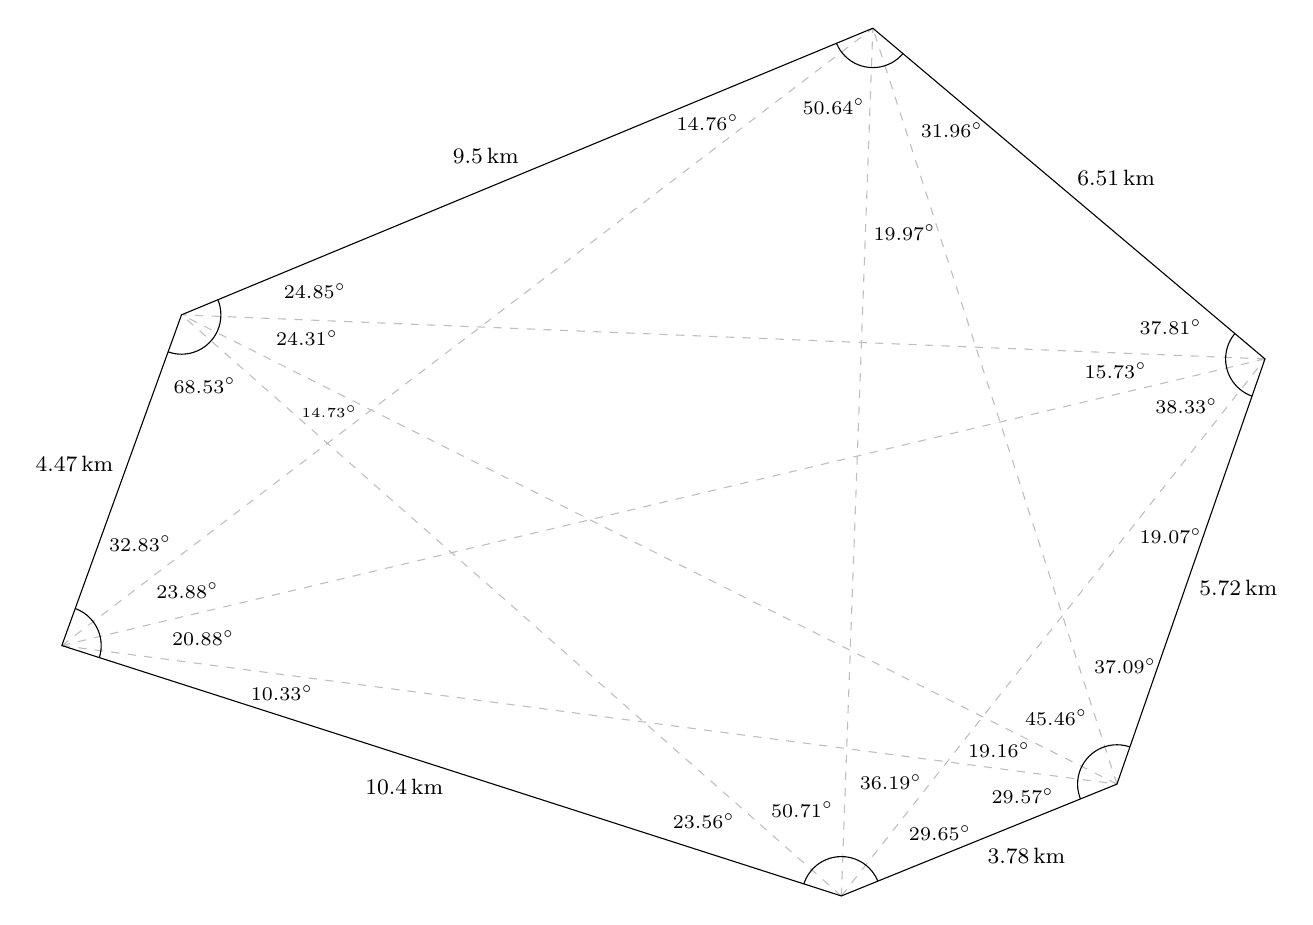
\begin{tikzpicture}
      \begin{footnotesize}

        \coordinate (A) at (0, 0);
        \coordinate (B) at (9.9, -3.18);
        \coordinate (C) at (13.4, -1.76);
        \coordinate (D) at (15.28, 3.64);
        \coordinate (E) at (10.3, 7.84);
        \coordinate (F) at (1.52, 4.2);

        \draw [dashed, color=gray!50]
        (A) -- (C)
        (A) -- (D)
        (A) -- (E)
        (B) -- (D)
        (B) -- (E)
        (B) -- (F)
        (C) -- (E)
        (C) -- (F)
        (D) -- (F);

        \draw (A)
        -- (B) node [midway, below left] {\SI{10.4}{\kilo\meter}}
        -- (C) node [midway, below right] {\SI{3.78}{\kilo\meter}}
        -- (D) node [midway, below right] {\SI{5.72}{\kilo\meter}}
        -- (E) node [midway, above right] {\SI{6.51}{\kilo\meter}}
        -- (F) node [midway, above left] {\SI{9.5}{\kilo\meter}}
        -- cycle node [midway, above left] {\SI{4.47}{\kilo\meter}};

        \begin{scriptsize}
          \newcommand{\lab}[3]{node [#1=#2] {\SI{#3}{\degree}}}
          \begin{scope}
            \clip (A) -- (B) -- (C) -- (D) -- (E) -- (F) -- cycle;

            \draw (A) circle (0.5cm) (A)
            \lab{above right}{-0.8cm and 2.3cm}{10.33}
            \lab{above right}{-0.1cm and 1.3cm}{20.88}
            \lab{above right}{0.5cm and 1.1cm}{23.88}
            \lab{above right}{1.1cm and 0.5cm}{32.83};

            \draw (F) circle (0.5cm) (F)
            \lab{below right}{0.7cm and -0.2cm}{68.53}
            node [below right=1.05cm and 1.425cm] {\tiny \SI{14.73}{\degree}}
            \lab{below right}{0.1cm and 1.1cm}{24.31}
            \lab{below right}{-0.5cm and 1.2cm}{24.85};

            \draw (E) circle (0.5cm) (E)
            \lab{below left}{1.0cm and 1.6cm}{14.76}
            \lab{below left}{0.8cm and 0cm}{50.64}
            \lab{below left}{2.4cm and -0.9cm}{19.97}
            \lab{below left}{1.1cm and -1.5cm}{31.96};

            \draw (D) circle (0.5cm) (D)
            \lab{below left}{-0.6cm and 0.7cm}{37.81}
            \lab{below left}{-0.05cm and 1.4cm}{15.73}
            \lab{below left}{0.4cm and 0.5cm}{38.33}
            \lab{below left}{2.05cm and 0.7cm}{19.07};

            \draw (C) circle (0.5cm) (C)
            \lab{above left}{1.3cm and -0.6cm}{37.09}
            \lab{above left}{0.65cm and 0.275cm}{45.46}
            \lab{above left}{0.2375cm and 1.0cm}{19.16}
            \lab{above left}{-0.35cm and 0.7cm}{29.57};

            \draw (B) circle (0.5cm) (B)
            \lab{above left}{0.6cm and -1.75cm}{29.65}
            \lab{above left}{1.25cm and -1.125cm}{36.19}
            \lab{above left}{0.9cm and 0.0cm}{50.71}
            \lab{above left}{0.75cm and 1.25cm}{23.56};
          \end{scope}
        \end{scriptsize}
      \end{footnotesize}
    \end{tikzpicture}
  \end{center}

  \vspace{0.5in}
  Find the area of the region. \emph{(Hint: can you use problem 1?)}
  \clearpage
\item \emph{Surveying a mountain:} You've been hired again, but this
  time you're surveying the region surrounding not a canyon but a
  mountain. Unfortunately, this makes it impossible to measure the
  angles between points on the far side---you can't see through the
  mountain, after all. The only thing you can measure are the angles
  between adjacent corners.

  \begin{center}
    \begin{tikzpicture}[x=0.85cm,y=0.85cm]
      \begin{footnotesize}

        \coordinate (A) at (-0.68, 14.79);
        \coordinate (B) at (8.26, 14.79);
        \coordinate (C) at (13.04, 9.55);
        \coordinate (D) at (8.72, 3.37);
        \coordinate (E) at (0.14, 0.37);
        \coordinate (F) at (-4.1, 7.01);

        \draw (A)
        -- (B) node [midway, above=0.1cm] {\SI{8.94}{\mile}}
        -- (C) node [midway, above right] {\SI{7.09}{\mile}}
        -- (D) node [midway, below right] {\SI{7.54}{\mile}}
        -- (E) node [midway, below right] {\SI{9.09}{\mile}}
        -- (F) node [midway, below left] {\SI{7.88}{\mile}}
        -- cycle node [midway, above left] {\SI{8.5}{\mile}};

        \begin{scope}
          \clip (A) -- (B) -- (C) -- (D) -- (E) -- (F) -- cycle;
          \draw (A) circle (0.5cm) (A) node [below right=0.4cm] {\SI{113.73}{\degree}};
          \draw (B) circle (0.5cm) (B) node [below left=0.4cm] {\SI{132.36}{\degree}};
          \draw (C) circle (0.5cm) (C) node [left=0.5cm] {\SI{102.68}{\degree}};
          \draw (D) circle (0.5cm) (D) node [above left=0.4cm] {\SI{144.23}{\degree}};
          \draw (E) circle (0.5cm) (E) node [above right=0.6cm and -0.2cm] {\SI{103.29}{\degree}};
          \draw (F) circle (0.5cm) (F) node [right=0.6cm] {\SI{123.71}{\degree}};
        \end{scope}
      \end{footnotesize}
    \end{tikzpicture}
  \end{center}

  \vspace{0.5in}
  Can you still find the area? \emph{(Hint: it may help to use
    triangles whose legs are aligned with one of the sides.)}
  \clearpage
\item \emph{Approximation:} Using any method you would like, obtain an
  approximation for the area of California. (At this scale,
  $\SI{1}{\square\inch} = \SI{29969}{\square\kilo\meter}$.)
  % Longitude: 114° 8' W to 124° 24' W
  % Latitude: 32° 30' N to 42° N
  %
  % Input Location Points
  % Latitude 1	 	Longitude 1
  % 32.5 N              119.266666667 W
  % Latitude 2	 	Longitude 2
  % 42 N                119.266666667 W
  %
  % Distance
  % (rounded to the nearest whole unit)
  % 1056 km
  %
  % Height of PDF: 6.1 inches
  %
  % 6.1 inches to 1056 km
  % 1 inch = 173.114754098 km
  % 1 square inch = 29968.718086411 square km
  \vspace{0.5in}
  \begin{center}
    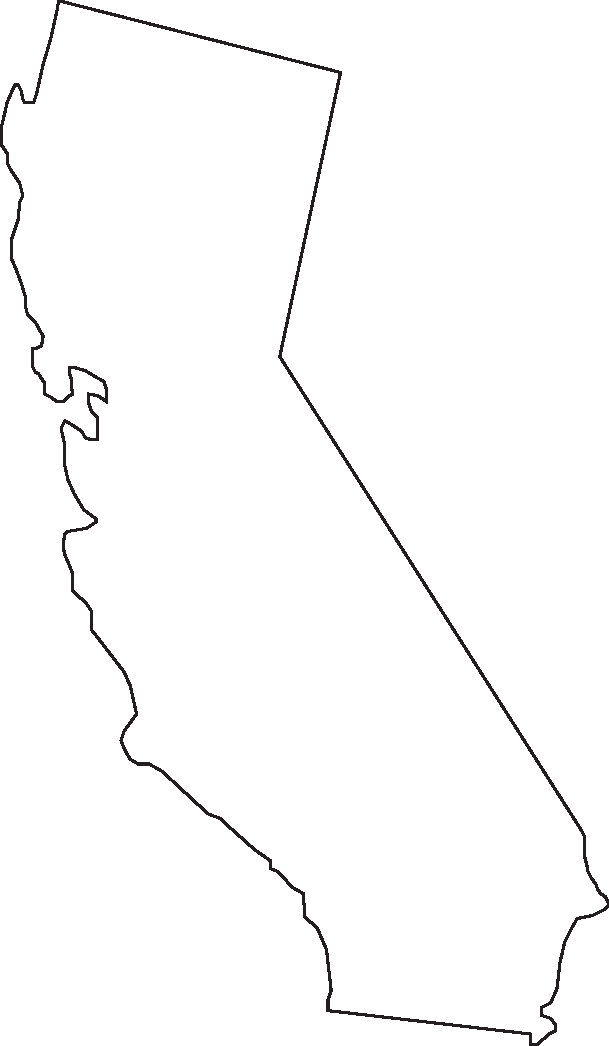
\includegraphics{california.pdf}
  \end{center}
  \vspace{0.5in}
\item \emph{Bonus:} What other ways can you think of to calculate
  these areas?
\end{enumerate}

\end{document}
